\chapter{Sorgenti del campo magnetico}

Nel capitolo precedente abbiamo trattato come un campo magnetico agisce su una carica, o un sistema di cariche, in movimento, tuttavia non abbiamo ancora parlato del legame esplicito tra il campo magnetico e le correnti che lo generano. \\

Di seguito andremo a trovare delle espressioni analoghe a quelle gia viste per il campo elettrico, relative, pero, al legame del campo magnetico con le cariche in moto. 

\section{Campo magnetico prodotto da una corrente}

L'analisi dei primi esperimenti sulle caratteristiche del campo magnetico prodotto da correnti in conduttori filiformi indusse Laplace a formulare una legge, nota come \emph{prima legge elementare di Laplace}, \mkeyword{prima legge elementare di Laplace} che esprime il campo magnetico prodotto da un tratto infinitesimo $ds$ di filo, percorso dalla corrente $i$, in un punto $P$ distante $r$ dall'elemento di filo

\begin{tcolorbox}[colback=yellow!10!white, colframe=orange!70!black, boxrule=0.8pt]
\begin{equation} \label{eq:legge_el_Laplace}
    d \mathbf{B} = \frac{\mu_0 i}{4 \pi} \frac{d \mathbf{s} \times \mathbf{u}_r}{r^2} = \frac{\mu_0 }{4 \pi} \frac{i \ d s}{r^2} \mathbf{u}_t \times \mathbf{u}_r 
\end{equation}
\end{tcolorbox}

Dove $\mathbf{u}_r$ è il versore della direzione orientata da $d s$ a $P$, $\mathbf{u}_t$ il versore tangente al filo per cui $d \mathbf{s} = ds \ \mathbf{u}_t$. 

\begin{figure}[h]
    \centering
    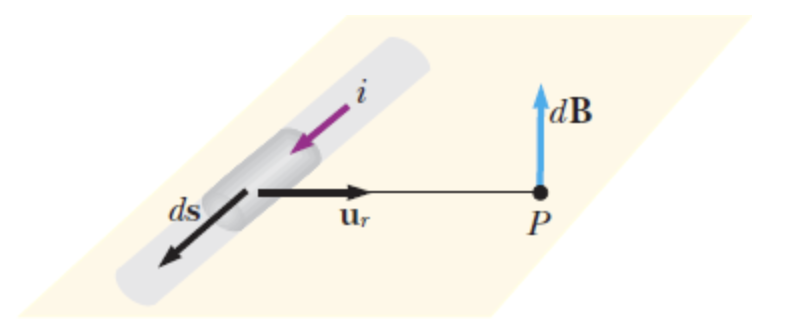
\includegraphics[width=0.7\linewidth]{figure/image43.png}
    \caption{Campo magnetico prodotto da un elemento di filo percorso da corrente}
    \label{fig:campo_magnetico_filo}
\end{figure}

Mentre $\mu_0$ è una costante che prende il nome di \emph{permeabilità nel vuoto} \mkeyword{permeabilità nel vuoto} e risulta

\begin{tcolorbox}[colback=yellow!10!white, colframe=orange!70!black, boxrule=0.8pt]
\begin{equation}
    \mu_0 = 1,26 \cdot 10^{-6} \ \frac{H}{m}
\end{equation}
\end{tcolorbox}

La \ref{eq:legge_el_Laplace} ha validità generale soltanto come strumento matematica di calcolo: sperimentalmente non è possibile misurare il contributo di un elemento infinitesimo del filo, che non può esistere da solo. \\

Ciò che ha significato fisico, e si può misurare, è la sovrapposizione dei contribui, cioè l'integrale di \ref{eq:legge_el_Laplace} esteso a un circuito chiuso $C$

\begin{tcolorbox}[colback=yellow!10!white, colframe=orange!70!black, boxrule=0.8pt]
\begin{equation}\label{eq:legge_Ampere-Laplace}
    \mathbf{B} = \frac{\mu_0 i}{4 \pi} \oint_C \frac{d\mathbf{s} \times \mathbf{u}_r}{r^2}
\end{equation}
\end{tcolorbox}

Questo risultato costituisce la \emph{legge di Ampère-Laplace}. \mkeyword{legge di Ampère-Laplace}\\

La \ref{eq:legge_Ampere-Laplace} dà in ogni punto dello spazio il campo magnetico dovuto a un circuito chiuso \emph{filiforme} fi forma qualunque. \\

Più in generale se il conduttore non è filiforme si considera un elemento lungo $d s$, di sezione $d \Sigma$, percorso da una corrente di intensità $\mathbf{j}$, quindi vale

\begin{equation*}
    d i \ d\mathbf{s} = \mathbf{j} \ d\Sigma \ ds = \mathbf{j} \  d \tau
\end{equation*}

Sostituendo nella \ref{eq:legge_el_Laplace} si ottiene 

\begin{tcolorbox}[colback=yellow!10!white, colframe=orange!70!black, boxrule=0.8pt]
\begin{equation}
    d\mathbf{B} = \frac{\mu_0 }{4 \pi} \frac{\mathbf{j} \times \mathbf{u}_r}{r^2} d\tau
\end{equation}
\end{tcolorbox}

e integrando in tutto il volume in cui $\mathbf{j}$ è diverso da zero si ottiene 

\begin{tcolorbox}[colback=yellow!10!white, colframe=orange!70!black, boxrule=0.8pt]
\begin{equation}\label{eq:legge_Ampere-Laplace_generale}
    \mathbf{B} = \frac{\mu_0 }{4 \pi} \int_{\tau} \frac{\mathbf{j} \times \mathbf{u}_r}{r^2} d\tau
\end{equation}
\end{tcolorbox}

Nel capitolo precedente abbiamo dedotto che il campo magnetico è solinoidale, adesso lo possiamo mostrare esplicitamente

\subsection{Divergenza del campo magnetico}

Riscriviamo la \ref{eq:legge_Ampere-Laplace_generale} nella forma 

\begin{equation*}
    \mathbf{B}(x,y,z) = \frac{\mu_0 }{4 \pi} \int_{\tau} \frac{\mathbf{j}(x',y',z') \times \mathbf{u}_r}{r^2} d\tau
\end{equation*}

Dove indichiamo con gli elementi non primati quelli che si riferiscono alla posizione del punto in cui andiamo a cercare il campo, mentre con gli elementi primati quelli che riferiscono ai punti del volume $\tau$. La divergenza di $\mathbf{B}$ è 

\begin{equation*}
    \nabla \cdot \mathbf{B} = \frac{\mu_0 }{4 \pi} \nabla \cdot \int_{\tau} \frac{\mathbf{j}(x',y',z') \times \mathbf{u}_r}{r^2} d\tau
\end{equation*}

Dato che la divergenza è calcolata rispetto alle coordinate $(x,y,z)$ mentre l'integrazione è fatta sulle coordinate $(x',y',z')$, per cui possiamo scrivere 

\begin{equation*}
    \nabla \cdot \mathbf{B} = \frac{\mu_0 }{4 \pi} \int_{\tau} \nabla \cdot \left[ \frac{\mathbf{j}(x',y',z') \times \mathbf{u}_r}{r^2} \right] d\tau = - \frac{\mu_0 }{4 \pi} \int_{\tau} \nabla \cdot \left[ \mathbf{j}(x',y',z') \times \nabla \left( \frac{1}{r} \right) \right] d\tau
\end{equation*}

Dove abbiamo posto $\mathbf{u}_r/r^2 = - \nabla(1/r)$. \\

Sfruttando l'identità $\nabla \cdot (\mathbf{a}\times \mathbf{b}) = \mathbf{b} \cdot \nabla \times \mathbf{a} - \mathbf{a} \times \nabla \times \mathbf{b}$ si ha:

\begin{align*}
    \nabla \cdot \left[ \mathbf{j}(x',y',z') \times \nabla \left( \frac{1}{r} \right) \right] = \\
    = \nabla \left( \frac{1}{r} \right) \cdot \nabla \times \mathbf{j} (x',y',z') - \mathbf{j}(x',y',z') \cdot \nabla \times \nabla \left( \frac{1}{r} \right) = 0
\end{align*}

dato che $\nabla$ opera sulle coordinate $(x,y,z)$, mentre $\mathbf{j}$ dipende da $(x',y',z')$, e che il rotore di un gradiente è identicamente nullo. \\

Applichiamo adesso la prima legge elementare di Laplace ad alcune configurazioni in cui la corrente percorre un conduttore filiforme di forma semplice.

\subsection{Filo rettilineo indefinito. Legge di Biot-Savart}

Consideriamo un filo conduttore rettilineo, di lunghezza $2a$, percorso dalla corrente $i$, e poniamoci nel piano mediano del filo nel punto $P$ distante $R$ dal filo. 

\begin{figure}[h]
    \centering
    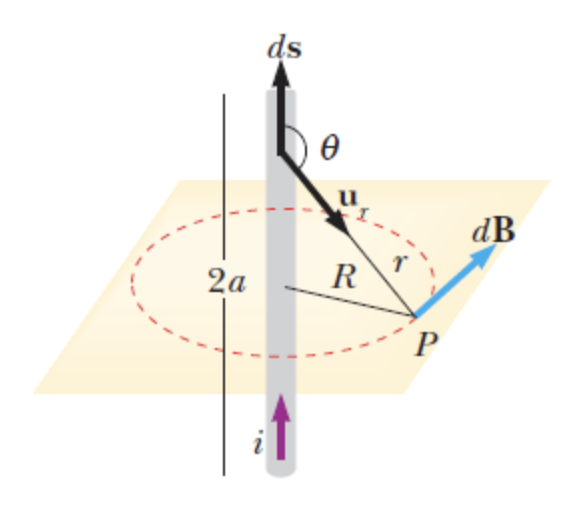
\includegraphics[width=0.5\linewidth]{figure/image44.png}
    \caption{Filo rettilineo}
    \label{fig:chapter_14_1}
\end{figure}

Un elemento di filo produce in $P$ il campo magnetico 

\begin{equation*}
    d \mathbf{B} = \frac{\mu_0 i}{4 \pi} \frac{d \mathbf{s} \times \mathbf{u}_r}{r^2} \implies dB = \frac{\mu_0 i}{4 \pi} \frac{ds \sin\theta}{r^2}
\end{equation*}

\'E conveniente andare ad esprimere $r$ e $ds$ in funzione di $\theta$. 

\begin{align*}
    r \sin (\pi - \theta) = r \sin\theta = R \implies \frac{1}{r^2} = \frac{\sin^2 \theta}{r^2},\\
    \text{tg}(\pi - \theta) = - \text{tg}\theta = \frac{R}{s} \implies ds = \frac{R d \theta}{\sin^2 \theta} , 
\end{align*}

\newpage

Quindi, sostituendo, si ottiene 

\begin{equation}
    dB = \frac{\mu_0 i}{4 \pi} \frac{\sin \theta \ d \theta}{R} =-\frac{\mu_0 i}{4 \pi} \frac{ d(\cos \theta) }{R}
\end{equation}

Possiamo trovare il campo generato da tutto il filo integrando 

\begin{equation*}
    B = -\frac{\mu_0 i}{4 \pi R} \int_{-\cos(\bar{\theta})}^{\cos(\bar{\theta})} d(\cos \theta) = \frac{\mu_0 i \cos(\bar{\theta})}{2 \pi R}
\end{equation*}

Allora, andando a sostituire $\cos(\bar{\theta})$ e sfruttando la simmetria per rotazione intorno all'asse passante per il filo si ottiene 

\begin{tcolorbox}[colback=yellow!10!white, colframe=orange!70!black, boxrule=0.8pt]
\begin{equation}
    \mathbf{B} = \frac{\mu_0 i a }{2 \pi R \sqrt{R^2 + a^2}} \mathbf{u}_{\phi}
\end{equation}
\end{tcolorbox}

In particolare se facciamo tendere la lunghezza $a$ all'infinito questa diventa 

\begin{tcolorbox}[colback=yellow!10!white, colframe=orange!70!black, boxrule=0.8pt]
\begin{equation} \label{eq:legge_Biot-Savart}
    \mathbf{B} = \frac{\mu_0 i }{2 \pi R } \mathbf{u}_{\phi}
\end{equation}
\end{tcolorbox}

Quest ultima è nota come \emph{legge di Biot-Savart} \mkeyword{legge di Biot-Savart} e afferma che il campo magnetico di un filo rettilineo indefinito dipende solo dalla distanza del filo, in modo inversamente proporzionale. 

\subsection{Spira circolare}

Passiamo ora a calcolare il campo magnetico sull'asse di una spira circolare di raggio $R$, percorsa da corrente $i$. 

\begin{figure} [h]
    \centering
    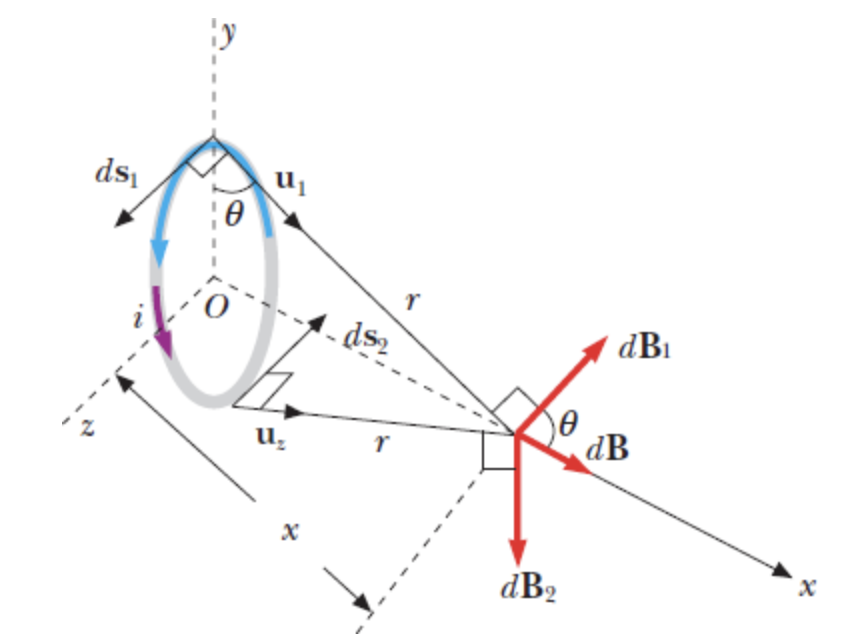
\includegraphics[width=0.6\linewidth]{figure/image45.png}
    \caption{Campo magnetico sull'asse di una sprira circolare}
    \label{fig:chapter_14_2}
\end{figure}

Nel punto $P$, distante $x$ da centro $O$ della spira, un elemento $d \mathbf{s}$ di spira genera il campo $d \mathbf{B}$ di modulo 

\begin{equation*}
    dB = \frac{\mu_0 i \ ds}{4 \pi r^2}
\end{equation*}

in quanto $d \mathbf{s}$ e $\mathbf{u}_r$ sono ortogonali. \\

La componente lungo l'asse $x$ vale 

\begin{equation*}
    dB_x = \frac{\mu_0 i \ ds}{4 \pi r^2} \cos \theta
\end{equation*}

dove $\theta$ è l'angolo che $d \mathbf{B}$ forma con l'asse $x$. Quando si considerano i contributi $d \mathbf{B}$ di tutti gli elementi $d \mathbf{s}$ che formano la spira, le componenti parallele all'asse si sommano, mentre quelle trasversali si elidono a due a due, per la simmetria del problema.

\begin{equation*}
    \mathbf{B} = \oint \frac{\mu_0 i}{4 \pi} \frac{\cos \theta}{r^2} ds \ \mathbf{u}_n = \frac{\mu_0 i}{4 \pi} \frac{\cos \theta}{r^2} 2 \pi R \ \mathbf{u}_n
\end{equation*}

Posto $r^2 = x^2 + R^2$ e $\cos \theta = R/r$ si ottiene 

\begin{tcolorbox}[colback=yellow!10!white, colframe=orange!70!black, boxrule=0.8pt]
\begin{equation} \label{eq:campo_spira_circolare}
    \mathbf{B} = \frac{\mu_0 i R^2}{2 r^3} \mathbf{u}_n = \frac{\mu_0 i R^2}{2 (x^2 + R^2)^{3/2}} \mathbf{u}_n
\end{equation}
\end{tcolorbox}

Allora nel centro della spira il campo è massimo e vale 

\begin{tcolorbox}[colback=yellow!10!white, colframe=orange!70!black, boxrule=0.8pt]
\begin{equation} 
    \mathbf{B} = \frac{\mu_0 i }{2 R} \mathbf{u}_n
\end{equation}
\end{tcolorbox}

Mentre per $x \to \infty$ il campo tende a zero.

\subsection{Solenoide rettilineo}

Un solenoide rettilineo è costituito da un filo conduttore avvolto a forma di elica cilindrica di piccolo passo. Sia $d$ la lunghezza del solenoide, $R$ il raggio, $N$ il numero totale di spire, $n = N/d$ il numero di spire per unità di lunghezza.

\begin{figure} [h]
    \centering
    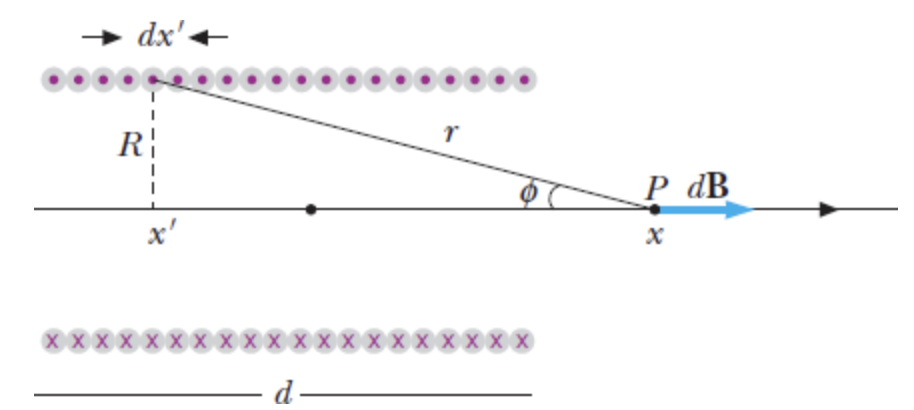
\includegraphics[width=0.6\linewidth]{figure/image46.png}
    \caption{Campo magnetico sull'asse di un solenoide rettilineo}
    \label{fig:chapter_14_3}
\end{figure}

Se le spire sono abbastanza fitte, così da poterle considerare distribuite con continuità, nel tratto di lunghezza $dx'$, di coordinata $x'$ rispetto ad un'origine $O$ sull'asse del solenoide, ce ne sono $ndx$. Il valore del campo magnetico in un punto $P$ sull'asse, di coordinata $x$, si calcola sfruttando la \ref{eq:campo_spira_circolare}, infatti il campo magnetico infinitesimo dato dalle spire nell'interavallo $dx'$ che si trovano nel punto $x'$ è data da 

\begin{equation*}
    dB = \frac{\mu_0 i R^2 n }{2r^3} dx'
\end{equation*}

\newpage

Per il calcolo del campo magnetico totale è conveniente introdurre la variabile $\phi$ e andare a esprimere $r$ e $dx'$ in funzione di questa: 

\begin{equation*}
    r = \frac{R}{\sin \phi} \quad , \quad \frac{R}{x - x'} = \text{tg}\phi \implies dx' = \frac{R d\phi }{\sin^2 \phi}
\end{equation*}

Sostituendo e integrando 

\begin{equation*}
    B = \frac{\mu_0 n i}{2} \int_{\phi_1}^{\phi_2} \sin \phi \ d \phi = \frac{\mu_0 n i}{2} (\cos \phi_1 - \cos \phi_2)
\end{equation*}

Esprimendo tutto in funzione della distanza $x$ dal centro del solenoide si ottiene

\begin{tcolorbox}[colback=yellow!10!white, colframe=orange!70!black, boxrule=0.8pt]
\begin{equation} 
    \mathbf{B} = \frac{\mu_0 n i}{2} \left[ \frac{d +2x}{\sqrt{(d+2x)^2 + 4R^2}} + \frac{d-2x}{\sqrt{(d-2x^2) + 4R^2}}  \right] \mathbf{u}_n
\end{equation}
\end{tcolorbox}

Si nota, allora, che il campo magnetico è massimo al centro della spira 

\begin{tcolorbox}[colback=yellow!10!white, colframe=orange!70!black, boxrule=0.8pt]
\begin{equation} 
    \mathbf{B}(O)= \mu_0 \ n i \frac{d}{\sqrt{d^2 + 4R^2}}  \mathbf{u}_n
\end{equation}
\end{tcolorbox}

Mentre nel centro di una spira estrema, cioè quando $x = \pm d/2$, si ha 

\begin{tcolorbox}[colback=yellow!10!white, colframe=orange!70!black, boxrule=0.8pt]
\begin{equation} 
    \mathbf{B}\left(\pm \frac{d}{2}\right)= \frac{\mu_0 \ n i}{2} \frac{d}{\sqrt{d^2 + R^2}}  \mathbf{u}_n
\end{equation}
\end{tcolorbox}

In particolare, se la lunghezza del solenoide è molto maggiore del raggio, il campo magetico in $O$ vale 

\begin{tcolorbox}[colback=yellow!10!white, colframe=orange!70!black, boxrule=0.8pt]
\begin{equation} 
    \mathbf{B}_{\infty}= \mu_0 \ n i \ \mathbf{u}_n
\end{equation}
\end{tcolorbox}

\newpage

\section{Azioni elettrodinamiche tra circuiti percorsi da corrente}

Calcoliamo la forza tra due circuiti percorsi da corrente. \\

\begin{figure}[h]
    \centering
    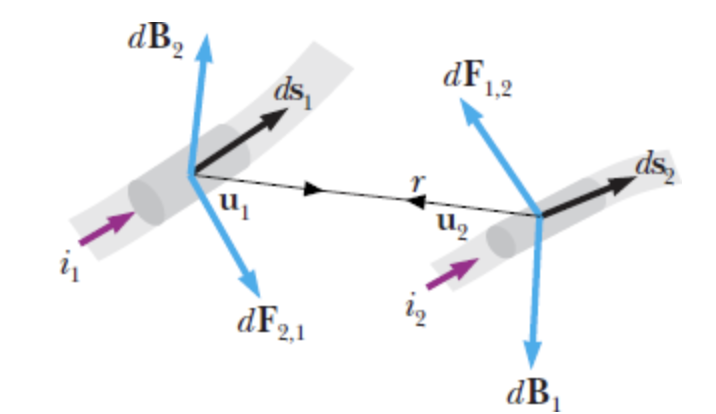
\includegraphics[width=0.6\linewidth]{figure/image47.png}
    \caption{Forza tra due tratti di circuito}
    \label{fig:chapter_14_4}
\end{figure}

Detti $d \mathbf{s}_1$ e $d \mathbf{s}_2$ gli elementi di filo dei circuiti e $i_1$ e $i_2$ le rispettive correnti. La forza $d \mathbf{F}_{1,2}$ agente sull'elemento $d\mathbf{s}_2$ a causa del campo magnetico $d \mathbf{B}_1$ prodotto da $d\mathbf{s}_1$ risulta

\begin{equation}
    d \mathbf{F}_{1,2} = i_2 \ d \mathbf{s}_2 \times d \mathbf{B}_1 = \frac{\mu_0 i_1 i_2}{4 \pi} \frac{ d \mathbf{s}_2 \times (d \mathbf{s}_1 \times \mathbf{u}_1)}{r^2}
\end{equation}

Mentre la forza esercitata da $d \mathbf{s}_2$ su $d \mathbf{s}_1$ è data da 

\begin{equation}
    d \mathbf{F}_{2,1} = \frac{\mu_0 i_1 i_2}{4 \pi} \frac{ d \mathbf{s}_1 \times (d \mathbf{s}_2 \times \mathbf{u}_2)}{r^2}
\end{equation}

Non è difficile trovare situazioni particolari in cui $d\mathbf{F}_{1,2} \neq - d\mathbf{F}_{2,1}$, in contrasto con il principio di azione e reazione; il fatto tuttavia non è preoccupante in quanto, come è stato notato, le leggi elementari di Laplace, considerate a sé, non si applicano a sistemi fisicamente realizzabili.\\

La forza risultante tra i due circuiti si ottiene con una doppia integrazione estesa ai due circuiti che tiene conto di tutte le coppie di elementi $d\mathbf{s}_1$ e $d \mathbf{s}_2$ tra i quali si esercitano le forze $d \mathbf{F}$:

\begin{tcolorbox}[colback=yellow!10!white, colframe=orange!70!black, boxrule=0.8pt]
\begin{equation} 
    \mathbf{F}_{1,2} = \frac{\mu_0 i_1 i_2}{4 \pi} \oint_1 \oint_2 \frac{d \mathbf{s}_2 \times (d\mathbf{s}_1 \times \mathbf{u}_1)}{r^2} \quad , \quad \mathbf{F}_{2,1} = \frac{\mu_0 i_1 i_2}{4 \pi} \oint_2 \oint_1 \frac{d \mathbf{s}_1 \times (d\mathbf{s}_2 \times \mathbf{u}_2)}{r^2}
\end{equation}
\end{tcolorbox}

\'E possibile dimostrare che 

\begin{equation}
    \mathbf{F}_{12} + \mathbf{F}_{21} = 0
\end{equation}

Quindi vale il principio di azione e reazione. 

\subsection{Forza tra due fili rettilinei}

Esaminiamo il caso di due fili rettilinei, percorsi rispettivamente dalle correnti $i_1$ e $i_2$, molto lunghi e abbastanza vicini da poter essere considerati indefiniti. \\

Se essi sono perpendicolari l'uno all'altro la forza tra i due fili è nulla: infatti ciascun filo risulta parallelo al campo magnetico prodotto dall'altro. \\

Consideriamo il caso in cui i due fili sono paralleli 

\begin{figure} [h]
    \centering
    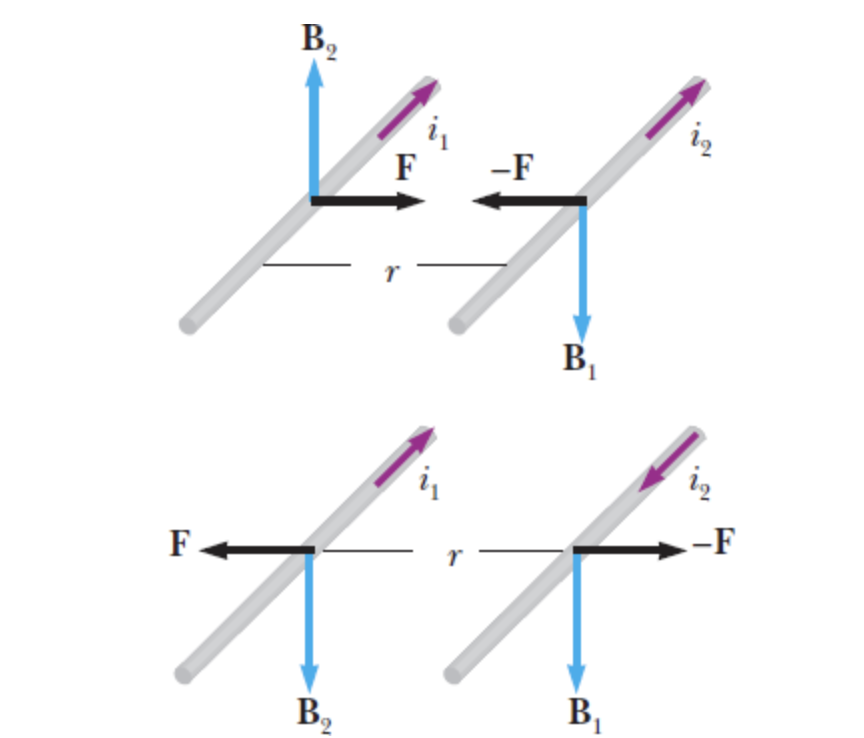
\includegraphics[width=0.5\linewidth]{figure/image48.png}
    \caption{Forza tra due fili indefiniti paralleli percorsi da corrente}
    \label{fig:chapter_14_5}
\end{figure}

Se i due fili, rispettivamente di lunghezza $l_1$ e $l_2$ e distanti $r$ sono paralleli, ciascun filo è perpendicolare al campo magnetico prodotto dall'altro, pertanto vale

\begin{equation}
    \mathbf{F}_{1,2} = i_2 \mathbf{l}_2 \times \mathbf{B}_1 \quad , \quad \mathbf{F}_{2,1} = i_1 \mathbf{l_1} \times \mathbf{B}_2 
\end{equation}

Le due forze, entrambe diretta secondo la congiungente dei fili, sono attrattive se le due correnti sono equiverse e repulsive se sono contrarie.\\
Il modulo della forza per unità di lunghezza di filo è data da 

\begin{tcolorbox}[colback=yellow!10!white, colframe=orange!70!black, boxrule=0.8pt]
\begin{equation}
    F_l = \frac{F_{1,2}}{l_2} = \frac{F_{2,1}}{l_1} = \mu_0 \frac{i_1 i_2}{2 \pi r}
\end{equation}
\end{tcolorbox}

avendo utilizzato la \ref{eq:legge_Biot-Savart} per il campo magnetico. 

\newpage 

\section{Legge di Ampère}

Sappiamo che nel caso generale vale la \ref{eq:legge_Ampere-Laplace_generale}, che, ponendo $r = |\mathbf{r} - \mathbf{r'}|$ dove $\mathbf{r}$ rappresenta la posizione dove stiamo calcolando il campo magnetico, mentre $\mathbf{r'}$ è la posizione di un particolare punto della sorgente del campo, diventa 

\begin{equation}
    \mathbf{B}(\mathbf{r}) = \frac{\mu_0}{4 \pi} \int_{\tau} \mathbf{j} (\mathbf{r'}) \times \frac{\mathbf{r} - \mathbf{r'}}{|\mathbf{r} - \mathbf{r'}|^3} d\tau
\end{equation}

In modo analogo a quanto fatto per il calcolo della divergenza del campo, si ha 

\begin{equation*}
    \mathbf{B}(\mathbf{r}) = - \frac{\mu_0}{4 \pi} \int_{\tau} \mathbf{j} (\mathbf{r}') \times \nabla\left( \frac{1}{|\mathbf{r} - \mathbf{r'}|} \right) d\tau
\end{equation*}

Utilizzando ora l'anticommutatività del prodotto vettoriale,

\begin{equation*}
    \mathbf a \times \mathbf b = - \mathbf b \times \mathbf a
\end{equation*}

segue che

\begin{equation*}
    \mathbf{B}(\mathbf{r})
    = \frac{\mu_0}{4 \pi} \int_{\tau}
    \nabla \left( \frac{1}{|\mathbf r - \mathbf r'|} \right)
    \times \mathbf{j}(\mathbf r') \, d\tau.
\end{equation*}

A questo punto si utilizza l'identità vettoriale

\begin{equation}
    \nabla \times (f \mathbf A)
    = (\nabla f) \times \mathbf A + f (\nabla \times \mathbf A).
\end{equation}

Ponendo

\begin{equation*}
f(\mathbf r)=\frac{1}{|\mathbf r - \mathbf r'|}, \qquad \mathbf A=\mathbf j(\mathbf r'),
\end{equation*}

e osservando che $\mathbf j(\mathbf r')$ dipende solo dalle coordinate primate e quindi risulta costante rispetto all'operatore $\nabla_{\mathbf r}$, si ha

\begin{equation*}
    \nabla \times \mathbf j(\mathbf r') = 0.
\end{equation*}

Segue dunque

\begin{equation*}
    \nabla \times \left( \frac{\mathbf j(\mathbf r')}{|\mathbf r - \mathbf r'|} \right)
    =
    \nabla \left( \frac{1}{|\mathbf r - \mathbf r'|} \right)
    \times \mathbf j(\mathbf r').
\end{equation*}

L'espressione del campo magnetico diventa quindi

\begin{equation*}
    \mathbf{B}(\mathbf{r})
    =
    \frac{\mu_0}{4 \pi}
    \int_{\tau}
    \nabla \times
    \left(
    \frac{\mathbf j(\mathbf r')}{|\mathbf r - \mathbf r'|}
    \right) d\tau.
\end{equation*}

Poiché l'operatore rotore agisce sulle variabili $\mathbf r$ mentre l'integrazione è estesa alle variabili primate $\mathbf r'$, esso può essere portato fuori dal segno di integrale:

\begin{equation} \label{eq:forma_util_legge_Ampère-Laplace}
    \mathbf{B}(\mathbf{r})
    =
    \frac{\mu_0}{4 \pi}
    \nabla \times
    \int_{\tau}
    \frac{\mathbf j(\mathbf r')}{|\mathbf r - \mathbf r'|} \, d\tau.
\end{equation}

Dopo queste prime operazioni iniziali, possiamo adesso passare al calcolo effettivo del rotore di $\mathbf{B}(\mathbf{r})$. \\

A partire dalla \ref{eq:forma_util_legge_Ampère-Laplace} si ha dunque

\begin{equation*}
    \nabla \times \mathbf B(\mathbf r)
    =
    \frac{\mu_0}{4\pi}\,
    \nabla \times \nabla \times
    \int_{\tau}\frac{\mathbf j(\mathbf r')}{|\mathbf r-\mathbf r'|}\,d\tau'
\end{equation*}

Per semplificare la notazione, introduciamo il campo ausiliario

\begin{equation*}
    \mathbf A(\mathbf r)\equiv \int_{\tau}\frac{\mathbf j(\mathbf r')}{|\mathbf r-\mathbf r'|}\,d\tau',
\end{equation*}

cosicché

\begin{equation}\label{eq:curlcurlA}
    \nabla \times \mathbf B(\mathbf r)
    =
    \frac{\mu_0}{4\pi}\,\nabla \times (\nabla \times \mathbf A)
\end{equation}

Usando l'identità vettoriale (valida per un campo vettoriale arbitrario $\mathbf A$)

\begin{equation}
    \nabla \times (\nabla \times \mathbf A)=\nabla(\nabla\cdot \mathbf A)-\nabla^2\mathbf A,
\end{equation}

la \ref{eq:curlcurlA} diventa

\begin{equation}\label{eq:step1}
    \nabla \times \mathbf B(\mathbf r)
    =
    \frac{\mu_0}{4\pi}\left[
    \nabla(\nabla\cdot \mathbf A)-\nabla^2\mathbf A
    \right].
\end{equation}

Poiché l'operatore $\nabla$ agisce sulle variabili non primate $\mathbf r$, mentre $\mathbf j(\mathbf r')$ dipende solo da $\mathbf r'$, si può scrivere

\begin{equation*}
    \nabla\cdot \mathbf A(\mathbf r)
    =
    \nabla\cdot \int_{\tau}\frac{\mathbf j(\mathbf r')}{|\mathbf r-\mathbf r'|}\,d\tau'
    =
    \int_{\tau}\mathbf j(\mathbf r')\cdot \nabla\!\left(\frac{1}{|\mathbf r-\mathbf r'|}\right)\,d\tau'
\end{equation*}

Segue quindi

\begin{equation}\label{eq:term_divA}
    \nabla(\nabla\cdot \mathbf A)
    =
    \nabla \int_{\tau}\mathbf j(\mathbf r')\cdot \nabla\!\left(\frac{1}{|\mathbf r-\mathbf r'|}\right)\,d\tau'
\end{equation}

Analogamente,

\begin{equation*}
    \nabla^2\mathbf A(\mathbf r)
    =
    \int_{\tau}\mathbf j(\mathbf r')\,\nabla^2\!\left(\frac{1}{|\mathbf r-\mathbf r'|}\right)\,d\tau'.
\end{equation*}

Sostituendo \ref{eq:term_divA} in \ref{eq:step1} otteniamo

\begin{equation}\label{eq:step2}
    \nabla \times \mathbf B(\mathbf r)
    =
    \frac{\mu_0}{4\pi}\,
    \nabla \int_{\tau}\mathbf j(\mathbf r')\cdot \nabla\!\left(\frac{1}{|\mathbf r-\mathbf r'|}\right)\,d\tau'
    -\frac{\mu_0}{4\pi}\int_{\tau}\mathbf j(\mathbf r')\,\nabla^2\!\left(\frac{1}{|\mathbf r-\mathbf r'|}\right)\,d\tau'
\end{equation}

A questo punto utilizziamo le identità (derivate dal fatto che la dipendenza è solo da $\mathbf r-\mathbf r'$)

\begin{equation}
    \nabla\!\left(\frac{1}{|\mathbf r-\mathbf r'|}\right)
    = -\,\nabla'\!\left(\frac{1}{|\mathbf r-\mathbf r'|}\right),
\end{equation}

e, in senso distribuzionale,

\begin{equation}\label{eq:laplacian_green}
    \nabla^2\!\left(\frac{1}{|\mathbf r-\mathbf r'|}\right)
    = -4\pi\,\delta(\mathbf r-\mathbf r').
\end{equation}

Sostituendo \ref{eq:laplacian_green} nel secondo integrale in \ref{eq:step2} si ottiene immediatamente

\begin{equation}
    -\frac{\mu_0}{4\pi}\int_{\tau}\mathbf j(\mathbf r')\,\nabla^2\!\left(\frac{1}{|\mathbf r-\mathbf r'|}\right)\,d\tau'
    =
    -\frac{\mu_0}{4\pi}\int_{\tau}\mathbf j(\mathbf r')\left[-4\pi\,\delta(\mathbf r-\mathbf r')\right]\,d\tau'
    =
    \mu_0\,\mathbf j(\mathbf r).
\end{equation}

Pertanto \ref{eq:step2} diventa

\begin{equation}\label{eq:step3}
    \nabla \times \mathbf B(\mathbf r)
    =
    \mu_0\,\mathbf j(\mathbf r)
    +\frac{\mu_0}{4\pi}\,
    \nabla \int_{\tau}\mathbf j(\mathbf r')\cdot \nabla\!\left(\frac{1}{|\mathbf r-\mathbf r'|}\right)\,d\tau'.
\end{equation}

Usando ora $\nabla(1/|\mathbf r-\mathbf r'|)=-\nabla'(1/|\mathbf r-\mathbf r'|)$, il termine integrale si riscrive come

\begin{equation}
    \nabla \int_{\tau}\mathbf j(\mathbf r')\cdot \nabla\!\left(\frac{1}{|\mathbf r-\mathbf r'|}\right)\,d\tau'
    =
    -\nabla \int_{\tau}\mathbf j(\mathbf r')\cdot \nabla'\!\left(\frac{1}{|\mathbf r-\mathbf r'|}\right)\,d\tau'.
\end{equation}

Integrando per parti rispetto alle variabili primate (trascurando i termini di superficie, nulli se $\mathbf j$ è confinata e/o decade sufficientemente rapidamente all'infinito), si ha

\begin{equation*}
    \int_{\tau}\mathbf j(\mathbf r')\cdot \nabla'\!\left(\frac{1}{|\mathbf r-\mathbf r'|}\right)\,d\tau'
    =
    -\int_{\tau}\frac{\nabla'\cdot \mathbf j(\mathbf r')}{|\mathbf r-\mathbf r'|}\,d\tau'
\end{equation*}

Quindi \ref{eq:step3} diventa

\begin{equation}\label{eq:ampere_general}
    \nabla \times \mathbf B(\mathbf r)
    =
    \mu_0\,\mathbf j(\mathbf r)
    +\frac{\mu_0}{4\pi}\,
    \nabla \int_{\tau}\frac{\nabla'\cdot \mathbf j(\mathbf r')}{|\mathbf r-\mathbf r'|}\,d\tau'.
\end{equation}

Nel caso magnetostatico (correnti stazionarie) vale l'equazione di continuità

\begin{equation*}
\frac{\partial \rho}{\partial t}+\nabla\cdot \mathbf j=0
\qquad\Rightarrow\qquad
\nabla\cdot \mathbf j=0,
\end{equation*}

e dunque anche $\nabla'\cdot \mathbf j(\mathbf r')=0$. Il secondo termine in \ref{eq:ampere_general} si annulla e si ottiene infine

\begin{tcolorbox}[colback=yellow!10!white, colframe=orange!70!black, boxrule=0.8pt]
\begin{equation} \label{eq:Legge_Ampere_locale}
    \nabla \times \mathbf B(\mathbf r)=\mu_0\,\mathbf j(\mathbf r),
\end{equation}
\end{tcolorbox}

che è la legge di Ampère in forma differenziale per la \mkeyword{Legge di Ampère locale} magnetostatica.\\

Una volta ottenuta la \ref{eq:Legge_Ampere_locale} possiamo ricavarne la corrispondente forma integrale applicando il teorema di Stokes.\\

Sia dunque $S$ una superficie regolare orientata, con versore normale $\mathbf n$, e sia $C=\partial S$ il suo bordo, orientato positivamente secondo la regola della mano destra rispetto a $\mathbf n$.
Integrando entrambi i membri della \ref{eq:Legge_Ampere_locale} su $S$ si ottiene

\begin{equation}\label{eq:Ampere_step_surface}
    \int_S (\nabla \times \mathbf B)\cdot \mathbf n\, d a
    =
    \mu_0 \int_S \mathbf j \cdot \mathbf n\, d a
\end{equation}

Per il teorema di Stokes,
\begin{equation}\label{eq:Stokes}
    \int_S (\nabla \times \mathbf B)\cdot \mathbf n\, d a
    =
    \oint_C \mathbf B \cdot d\mathbf{s}
\end{equation}

dove $d\mathbf{s}$ è l'elemento di linea orientato lungo $C$.
Sostituendo \ref{eq:Stokes} in \ref{eq:Ampere_step_surface} segue quindi

\begin{equation}\label{eq:Ampere_integrale_flux}
    \oint_C \mathbf B \cdot d\mathbf{s}
    =
    \mu_0 \int_S \mathbf j \cdot \mathbf n\, d a
\end{equation}

Osserviamo ora che l'integrale di superficie del flusso di densità di corrente fornisce la corrente totale concatenata con la curva $C$, cioè

\begin{equation}\label{eq:def_Iconc}
    i \equiv \int_S \mathbf j \cdot \mathbf n\, d a
\end{equation}

Pertanto la \ref{eq:Ampere_integrale_flux} può essere riscritta nella forma più usuale

\begin{tcolorbox}[colback=yellow!10!white, colframe=orange!70!black, boxrule=0.8pt]
\begin{equation}\label{eq:Ampere_integrale}
    \oint_C \mathbf B \cdot d\mathbf{s} = \mu_0\, i
\end{equation}
\end{tcolorbox}

che è la \emph{legge di Ampère} \mkeyword{Legge di Ampère}in forma integrale per la magnetostatica.\\

Si noti inoltre che, in regime stazionario, la condizione $\nabla\cdot \mathbf j = 0$ garantisce che la corrente concatenata $i$ non dipenda dalla particolare superficie $S$ scelta, purché abbia bordo $C$: infatti, se $S_1$ e $S_2$ hanno lo stesso bordo $C$, la superficie chiusa $S_1\cup (-S_2)$ racchiude un volume $V$ e, per il teorema della divergenza,
\[
\int_{S_1}\mathbf j\cdot \mathbf n\,da-\int_{S_2}\mathbf j\cdot \mathbf n\,da
=
\int_{\partial V}\mathbf j\cdot \mathbf n\,da
=
\int_V (\nabla\cdot \mathbf j)\,d\tau
=0
\]
da cui $\int_{S_1}\mathbf j\cdot \mathbf n\,da=\int_{S_2}\mathbf j\cdot \mathbf n\,da$.
Di conseguenza anche il membro sinistro della \ref{eq:Ampere_integrale} è ben definito e dipende solo dalla curva $C$.\\

Quella riportata sopra è una dimostrazione \emph{molto} formale della legge di Ampère e da questa non si riesce a comprendere pienamente il significato fisico della legge stessa (in particolare cosa si intende quando si parla di "correnti concatenate"). Si consiglia pertanto al lettore, prima di proseguire, di consultare anche altri testi, nei quali è spesso presentata una dimostrazione più euristica.
